
\chapter{System Analysis and Design}
This chapter describes the study, analysis and design of the system. It highlights the identified requirements and Architectural design of the system.

\section{Overview of the system}
The system designed in this project is aimed at having students’ results stored and managed on a blockchain network. The management of the results on a blockchain network ensures more security compared to the traditional centralized systems. \\~\\
The system uses Ethereum which is a platform that allows creation of blockchain networks. For this project, Ganache is used as the local blockchain network on a user computer. The user gains access to the network using browser extension known as MetaMask. Each transaction that involves adding something to the blockchain network costs a given amount of ether which is a currency used to transact on the Ethereum network.

\begin{figure}[!h]
\centering
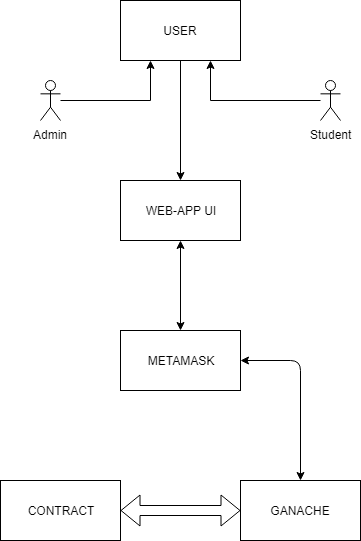
\includegraphics[scale=0.7]{images/simple_system.png}
\caption{Simple system Architecture}
\end{figure}

\newpage
\section{System Analysis}
\subsection{Data Analysis}
From the data retrieved during the research process, we found that the present system handling students’ records is prone to a number of errors and weaknesses.\\~\\
The current system handling students’ results at Makerere University does not have a limit to the number of times a student can do a course as opposed to the actual policy by the University where a student is meant to sit for exams in a course not more than three times.\\~\\
Another discovery from the data received was that the present-day system handling students’ results at Makerere University can accept an input of a percentage figure greater than 100\%.

\subsection{User Requirements}
Below are the user requirements for the blockchain results handler.
\begin{itemize}
\item Allow an administrative assistant enter students’ results.
\item Allow students to access their results without being able to change them.
\item Allow employers gain access to job applicants' past academic results. 
\end{itemize}

\subsection{Functional Requirements}
The functional requirements specify what the system is expected to do. These include the following;
\begin{itemize}
\item Provide verification of a user.
\item Ensure that the students’ results are not altered.
\end{itemize}


\subsection{Non Functional Requirements}
The non-functional requirements describe the behavior of the system, and these include:
\begin{itemize}
\item The system must verify any addition to the blockchain.
\item The system must notify the system administrator incase of any unauthorized transactions.
\end{itemize}
\subsection{System Requirements}
The system is built with a foundation on the ethereum network which is a platform that enables building of blockhain based smart contracts. MetaMask is a browser extension required for the system to allow a user access the ethereum blockchain network. All these have to be accessed on a Personal Computer with a browser e.g. google chrome, mozilla firefox among others.

\section{System Design}
This section includes a detailed description of the system’s architecture, components, modules, interfaces, and data for a system to satisfy the specified requirements. It describes the design and development process of the application using a use case diagram to explain how the actors will interact with the system and data flow diagrams to show how data will move in and out of the system.  

\subsection{System Architecture}
The system consists of the following major components:

\begin{itemize}
\item A blockchain network built on the Ethereum platform.
\item A PC that is used to access the blockchain network.
\item A user interface that allows a user to access the services of the system like adding to the chain, viewing results, among others.
\end{itemize}

\subsubsection{Class Diagram}
This is a static structure diagram that describes the structure of a system by showing the system's classes for example the student, Academic registrar, among others. It also shows their attributes, operations (or methods), and the relationships among objects.

\begin{figure}[!h]

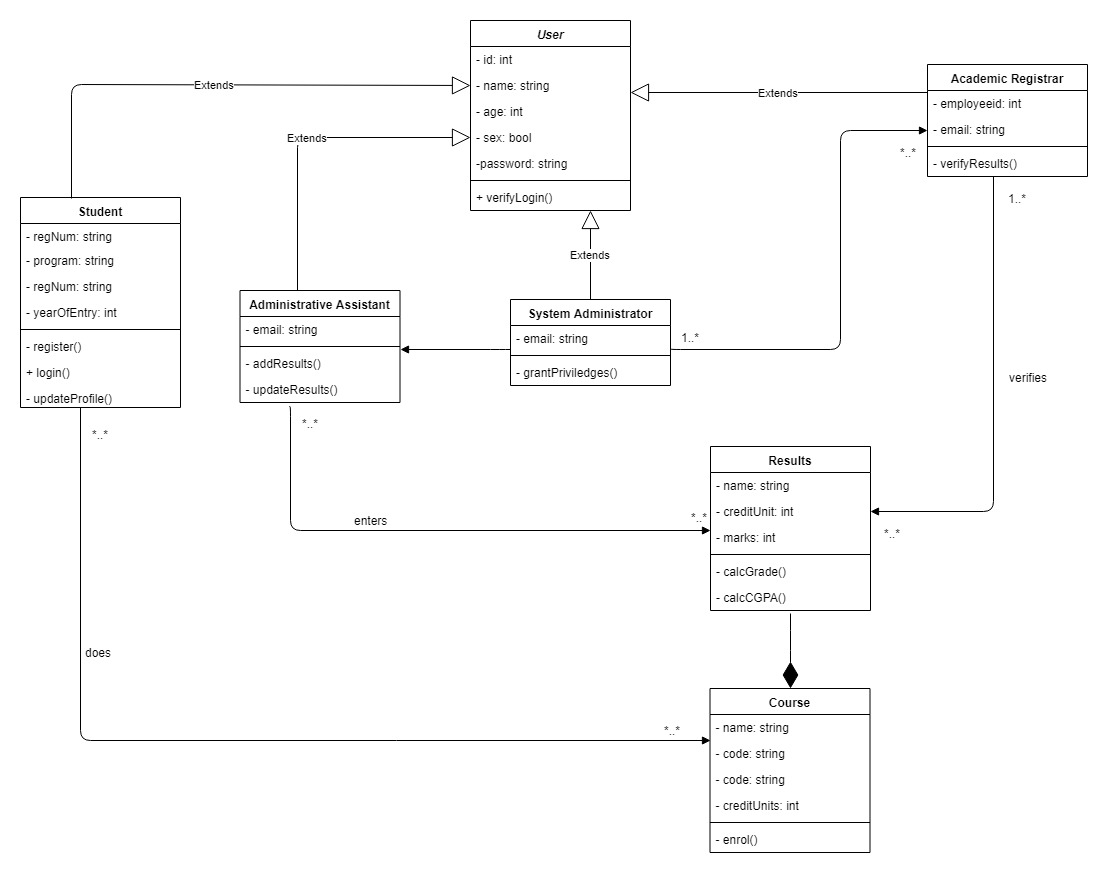
\includegraphics[scale=0.4]{images/class.jpg}
\caption{Class diagram}
\end{figure}


\subsubsection{Use Case Diagram}
This is a high level description of the different types of users of the system and how they interact with it. A use case diagram provides a simplified graphical representation of the system’s functionalities.

\begin{figure}[!h]
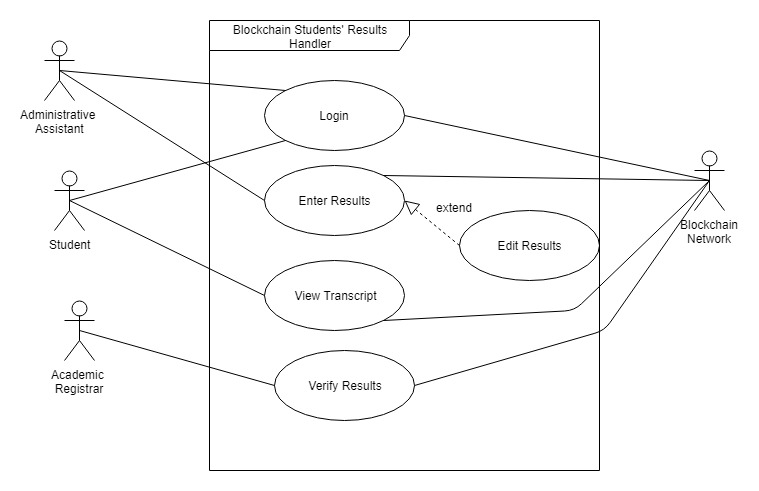
\includegraphics[scale=0.5]{images/Usecase.jpg}
\caption{Use Case diagram}
\end{figure}

\newpage
\subsubsection{Context Diagram}
This gives an overview of the entire system. In this diagram, there is only one process that represent the entire system. The purpose of this diagram is to display the expected inputs and outputs from the system to and from various entities. Shown in the diagram below is how various entities like students interact with the system.

\begin{figure}[!h]
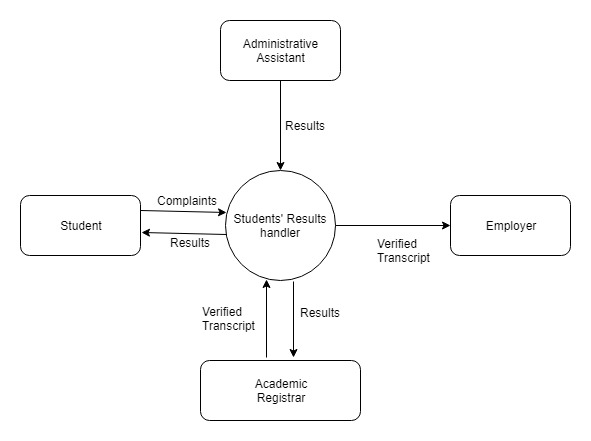
\includegraphics[scale=0.7]{images/context.jpg}
\caption{Context diagram}
\end{figure}

\subsection{Design Constraints}
Accessing the blockchain network requires reliable internet connectivity.\\

One needs to have the MetaMask browser extension installed on their browsers in order to access the blockchain network.\\

Writing to the blockchain costs gas. Gas in the context of Ethereum is a unit and a measurement for the computing power that is needed to execute certain operations in the Ethereum Virtual Machine (EVM).\\

The developers were limited to only ten virtual accounts to simulate actual accounts during development.\\


\textbf{Assumptions}\\
Some assumptions were made during the design and development of the system which include;\\

The end-user is willing to learn and adopt to the technology that may be new to him/her.\\

Users always have good internet reception.\\

Users are familiar with common internet browsers and file extensions for these browsers.\\

Scalability of the system will not negatively affect the application’s speed and reliability.\\

\subsection{Design Methodology}
We used the Agile software development (ASD) methodology. This methodology involves adaptive planning, evolutionary development, early delivery, and continual improvement. It also encourages rapid and flexible response to change. We focused on keeping code simple and testing often. This helped us to minimize risks such as bugs, cost overruns and the changing requirements.

\subsection{Graphical User Interface (GUI) Design}
This section provides the detailed design of the system and subsystem inputs and outputs relative to the user.

\subsubsection{Inputs}
\textbf{Ethereum network password:} the users’ password is required to create an account on the Ethereum network.  If the user is logging in on a different device from a previous one that was used to access the network, they’ll have to enter the seed phrase generated for them by the platform. \\

\textbf{Results:} When an administrative assistant logs into the system, he/she can enter the students’ results.

\subsubsection{Outputs}
\textbf{Testimonial:} before the results are forwarded to the blockchain, a student can access the system and view his/her progressive results.\\

\textbf{Transcript:} On accessing the platform, a student can view his transcript which can be printed as a pdf. An employer who would like to view an applicant’s past results can also access the network and view the same transcript.\\

\subsection{External Interfaces}

\subsubsection{Hardware Interfaces}
To fully access the functionality of this system, a user is required to have Computer with an internet browser(like google chrome, mozilla firefox, among others) with the MetaMask browser extension installed. 

\subsubsection{Software Interfaces}
The functionalities of the external interfaces were developed using web-based scripting langauages like PHP, JavaScript and the blockchain network built on the ethereum platform.

\subsubsection{Communication Interfaces}
The student details handled by the system are stored on an online sql database. The fully processed and verified transcript is stored on the blockchain built on the ethereum platform.

\subsubsection{User Interfaces}
Users navigate through the application using a windowed GUI. This involves clicking using a mouse, dragging and dropping among other manoeuvres possible with a windowed GUI.